\documentclass[11pt,a4paper,notitlepage]{exam}
\usepackage[utf8]{inputenc}
\usepackage{graphicx, wrapfig}

\usepackage{amsmath}
\usepackage{amsthm}
\usepackage{amssymb}
\usepackage{mathtools}

\renewcommand*{\proofname}{Prova}
% bold math
\usepackage{amsbsy}

% draw pictures (and graphs)
\usepackage{tikz}

% \usepackage[usenames,dvipsnames,svgnames,table]{xcolor}

% code in latex
\definecolor{dkgreen}{rgb}{0,0.6,0}
\definecolor{gray}{rgb}{0.5,0.5,0.5}
\definecolor{mauve}{rgb}{0.58,0,0.82}
\definecolor{newink}{rgb}{0,0.1,0.25}
\usepackage{caption}
\usepackage{listings}
\lstset{frame=tb,
  language=Python,
  aboveskip=3mm,
  belowskip=3mm,
  showstringspaces=false,
  columns=flexible,
  basicstyle={\small\ttfamily},
  numbers=none,
  numberstyle=\tiny\color{gray},
  keywordstyle=\color{blue},
  commentstyle=\color{dkgreen},
  stringstyle=\color{mauve},
  breaklines=true,
  breakatwhitespace=true,
  tabsize=3
}


\usepackage{multirow}

% definition equal
\newcommand\eqdef{\mathrel{\overset{\makebox[0pt]{\mbox{\normalfont\tiny\sffamily def}}}{=}}}

% independence equal
\newcommand\eqindep{\mathrel{\overset{\makebox[0pt]{\mbox{\normalfont\tiny\sffamily indep}}}{=}}}


% independent and identically distributed equal
\newcommand\eqiid{\mathrel{\overset{\makebox[0pt]{\mbox{\normalfont\tiny\sffamily i.i.d.}}}{=}}}

% * to cdot
\mathcode`\*="8000
{\catcode`\*\active\gdef*{\cdot}}

% pseudo-code
\usepackage[portuguese, linesnumbered]{algorithm2e}
\newcommand\Recebe{\leftarrow}
\newcommand\Comment{\vartriangleright}
\SetKw{Devolva}{devolva}
% Example:
% \paragraph{}
% \SetAlgoNoLine
% \textsc{Título-Do-Algoritmo}($A, n$)\\
% \begin{algorithm}[H]
%   \Devolva $A$
% \end{algorithm}
%

% pair ceil
\DeclarePairedDelimiter{\ceil}{\lceil}{\rceil}

% pair ceil
\DeclarePairedDelimiter{\floor}{\lfloor}{\rfloor}

% images
\usepackage{graphicx}
\graphicspath{ {./} }
% use: \includegraphics[scale=1]{image}


\setlength{\parindent}{3em}
\setlength{\parskip}{0.5em}

\begin{document}
% \SetAlgoNoLine
\begin{center}
%NOME E NUSP
Nome: \hphantom{xxx} NUSP: \\
%CURSO
Curso: Bacharelado em Ciência da Computação\\
%MATÉRIA
MAC0320 - Introdução à Teoria dos Grafos
\paragraph{}
\textbf{LISTA ?}
\end{center}

\paragraph*{E42.} Exemplo de enunciado.
\begin{proof}
 
  Exemplo de prova
\begin{align*}
  2 * |A(G)| &= \sum_{w \in V(G)} g(w)\\ &< n + \sum_{w \in V(G) \setminus \{u, v\}} g(w)\\
                                      &= 2*\Big(\frac{(n - 1)(n - 2)}{2} + 2\Big)\\
                                      &= 2*|A(G)|
\end{align*}
\end{proof}

Exemplo de grafo
\begin{center}
  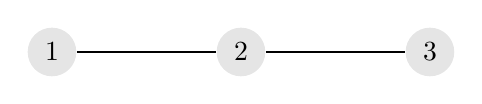
\begin{tikzpicture}
      [scale=.8,auto=left,every node/.style={circle,fill=gray!20}]
      \node (n1) at (0,0)  {1};
      \node (n2) at (3,0)  {2};
      \node (n3) at (6,0)  {3};
      \foreach \from/\to in {n1/n2, n2/n3}
        \draw (\from) -- (\to);   
    \end{tikzpicture}    
\end{center}

\end{document}
















